% IMPORTANT! In order for the document to compile, one needs to use XeLaTeX or LuaLaTeX as compiler. This can be done in  Overleaf by Menu -> Settings -> Compiler -> Choose XeLaTeX/LuaLaTeX
\documentclass[t,24pt,aspectratio=169]{beamer}

\usepackage{KUstyle}
\usepackage[style=authortitle,backend=biber]{biblatex}
\usepackage[]{float}
\usepackage{multicol} % Package for multiple coloumns

\addbibresource{../report/references/ref.bib}


%\toplinje{Master's thesis} % The text at top. Remove the command if no text is desired

\begin{document}

% The first slide. One can for instance change the main title, the subtitle, speaker, KU-unit and date
{
\setbeamertemplate{background}{
\includegraphics[width=\paperwidth,height=\paperheight]{KU/forside.pdf}}
\begin{frame}
    \begin{textblock*}{\textwidth}(0\textwidth,0.1\textheight)
        \begin{beamercolorbox}[wd=7.8cm,ht=7.3cm,sep=0.5cm]{hvidbox}
            \fontsize{5}{10}\fontfamily{ptm}\selectfont \textls[200]{UNIVERSITY OF COPENHAGEN}
            \noindent\textcolor{KUrod}{\rule{6.8cm}{0.4pt}}
        \end{beamercolorbox}
    \end{textblock*}
    \begin{textblock*}{\textwidth}(0\textwidth,0.1\textheight)
        \begin{beamercolorbox}[wd=7.8cm,sep=0.5cm]{hvidbox}
            \Huge \textcolor{KUrod}{Master's thesis}
            \vspace{0.5cm}
            \par
            \Large Implementation of a type-safe
            generalized syntax-directed editor
            \vspace{0.5cm}
            \par
            \normalsize Sune Skaanning Engtorp
            \vspace{0.3cm}
            \par
            \footnotesize Advisor: Hans Hüttel
        \end{beamercolorbox}
    \end{textblock*}
    \begin{textblock}{1}(6.3,11.38)
        
\includegraphics[width=1cm]{KU/KU-logo.png}
    \end{textblock}
\end{frame}
}

\begin{frame}[hvid]
    \frametitle{Agenda}

    \begin{itemize}
        \item Motivation and background
        \item Goal of the project
        \item Conclusion
        \item Background
        \item Implementation
        \item Editor examples
        \item Questions
    \end{itemize}
\end{frame}

\begin{frame}[hvid]
    \frametitle{Motivation and background}
    \begin{itemize}
        \item Structure editors
              \begin{itemize}
                  \item Avoid syntax errors
                  \item (Arguably) Improved code overview
                  \item With ability to support
                        \begin{itemize}
                            \item Typed holes
                            \item Context-sensitive syntax
                        \end{itemize}
              \end{itemize}
    \end{itemize}
\end{frame}


\begin{frame}[hvid]
    \frametitle{Motivation and background (Continued)}

    \begin{multicols}{2}
        \begin{itemize}
            \item Cornell Program Synthesizer (1981)\footcite{timtom81}

        \end{itemize}
        \vfill\null
        \columnbreak
        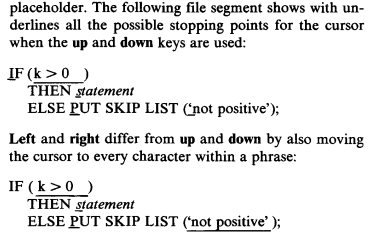
\includegraphics[width=0.4\textwidth]{img/cornell-ex.png}
    \end{multicols}
\end{frame}

\begin{frame}[hvid]
    \frametitle{Motivation and background (Continued)}

    \begin{multicols}{2}
        \begin{itemize}
            \item Hazel programming environment (2019)\footcite{omar}

        \end{itemize}

        \columnbreak
        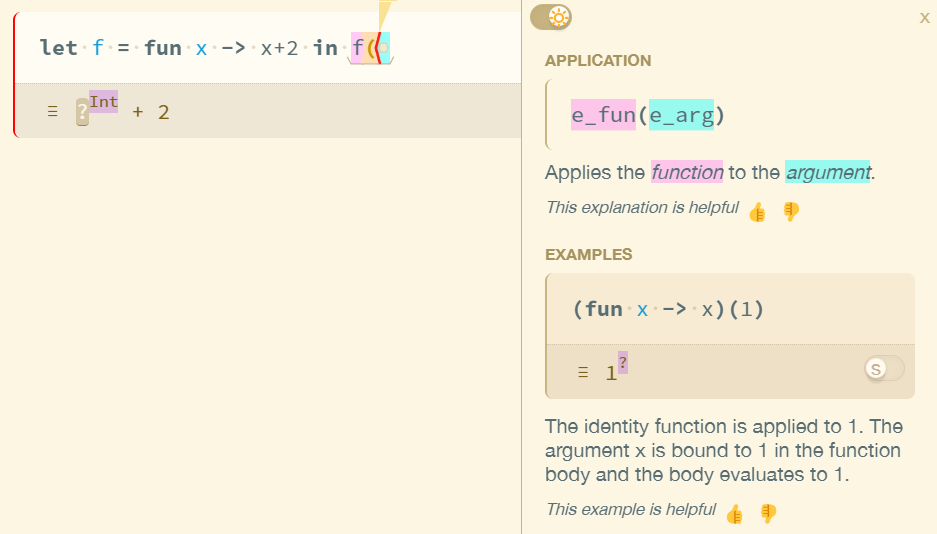
\includegraphics[width=0.5\textwidth]{img/hazel-ex.png}
    \end{multicols}
\end{frame}

\begin{frame}[hvid]
    \frametitle{Motivation and background (Continued)}

    \begin{multicols}{2}
        \begin{itemize}
            \item<1-> Type-Safe Structure Editor Calculus\footcite{godiksen}
            \item<2-> Implemented by a group of UCPH students\footcite{KU-bach}
            \item<3-> Generalized by a group of AAU students\footcite{aalborg}

        \end{itemize}

        \columnbreak
        \includegraphics<2->[width=0.5\textwidth]{img/ku-editor-ex.png}
    \end{multicols}
\end{frame}

\begin{frame}[hvid]
    \frametitle{Goal of the Project}
    \setbeamercovered{transparent}
    \begin{itemize}
        \item Implement an editor based on the generalized calculus
        \item Criteria for a good implementation:
              \begin{itemize}
                  \pause
                  \item Editing the abstract syntax of any program directly
                        \pause
                  \item Generic editing
                        \pause
                  \item Handling context-sensitive syntax
                        \pause
                  \item Multiple views of code being edited
                        \pause
                  \item Non-challenging way of specifying syntax
              \end{itemize}
              \pause
        \item Minimum viable product:
              \begin{itemize}
                  \pause
                  \item Editing the abstract syntax of any program directly
                        \pause
                  \item Generic editing
              \end{itemize}

    \end{itemize}
    \setbeamercovered{invisible}
\end{frame}

\begin{frame}[hvid]
    \frametitle{Picking good language examples}
    \begin{itemize}
        \item What makes a good set of examples?
              \begin{itemize}
                  \item Different paradigms and purposes:
                        \begin{itemize}
                            \item General purpose programming language
                            \item Domain-specific language
                            \item Markup language
                        \end{itemize}
                  \item Popular (present in GitHub top 30 ranking\footfullcite{prog-lang-metrics})
              \end{itemize}
              \pause
        \item Examples:
              \begin{itemize}
                  \item C
                  \item SQL
                  \item \LaTeX
              \end{itemize}
    \end{itemize}
\end{frame}

\begin{frame}[hvid]
    \frametitle{Picking good language examples (Continued)}

    \begin{multicols}{2}
        \begin{itemize}
            \item A C program with syntax errors

        \end{itemize}
        \vfill\null
        \columnbreak
        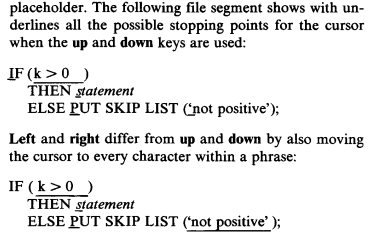
\includegraphics[width=0.4\textwidth]{img/cornell-ex.png}
    \end{multicols}
\end{frame}

\begin{frame}[hvid]
    \frametitle{Picking good language examples (Continued)}

    \begin{multicols}{2}
        \begin{itemize}
            \item A SQL query with syntax

        \end{itemize}
        \vfill\null
        \columnbreak
        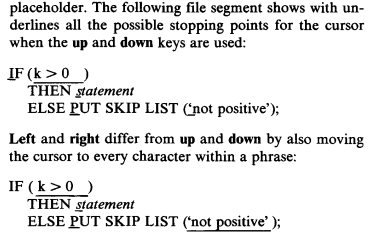
\includegraphics[width=0.4\textwidth]{img/cornell-ex.png}
    \end{multicols}
\end{frame}

\begin{frame}[hvid]
    \frametitle{Picking good language examples (Continued)}

    \begin{multicols}{2}
        \begin{itemize}
            \item A \LaTeX document with syntax errors

        \end{itemize}
        \vfill\null
        \columnbreak
        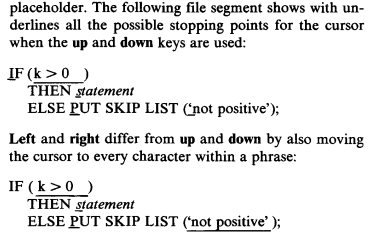
\includegraphics[width=0.4\textwidth]{img/cornell-ex.png}
    \end{multicols}
\end{frame}


\begin{frame}[hvid]
    \frametitle{Conclusion of the project}
    \begin{itemize}
        \item MVP has been achieved
        \item Conditional expressions have been implemented after submission
        \item Still missing (wrt. criteria for a good implementation):
              \begin{itemize}
                  \item Handling context-sensitive syntax
                  \item Views of code being edited
              \end{itemize}
    \end{itemize}
    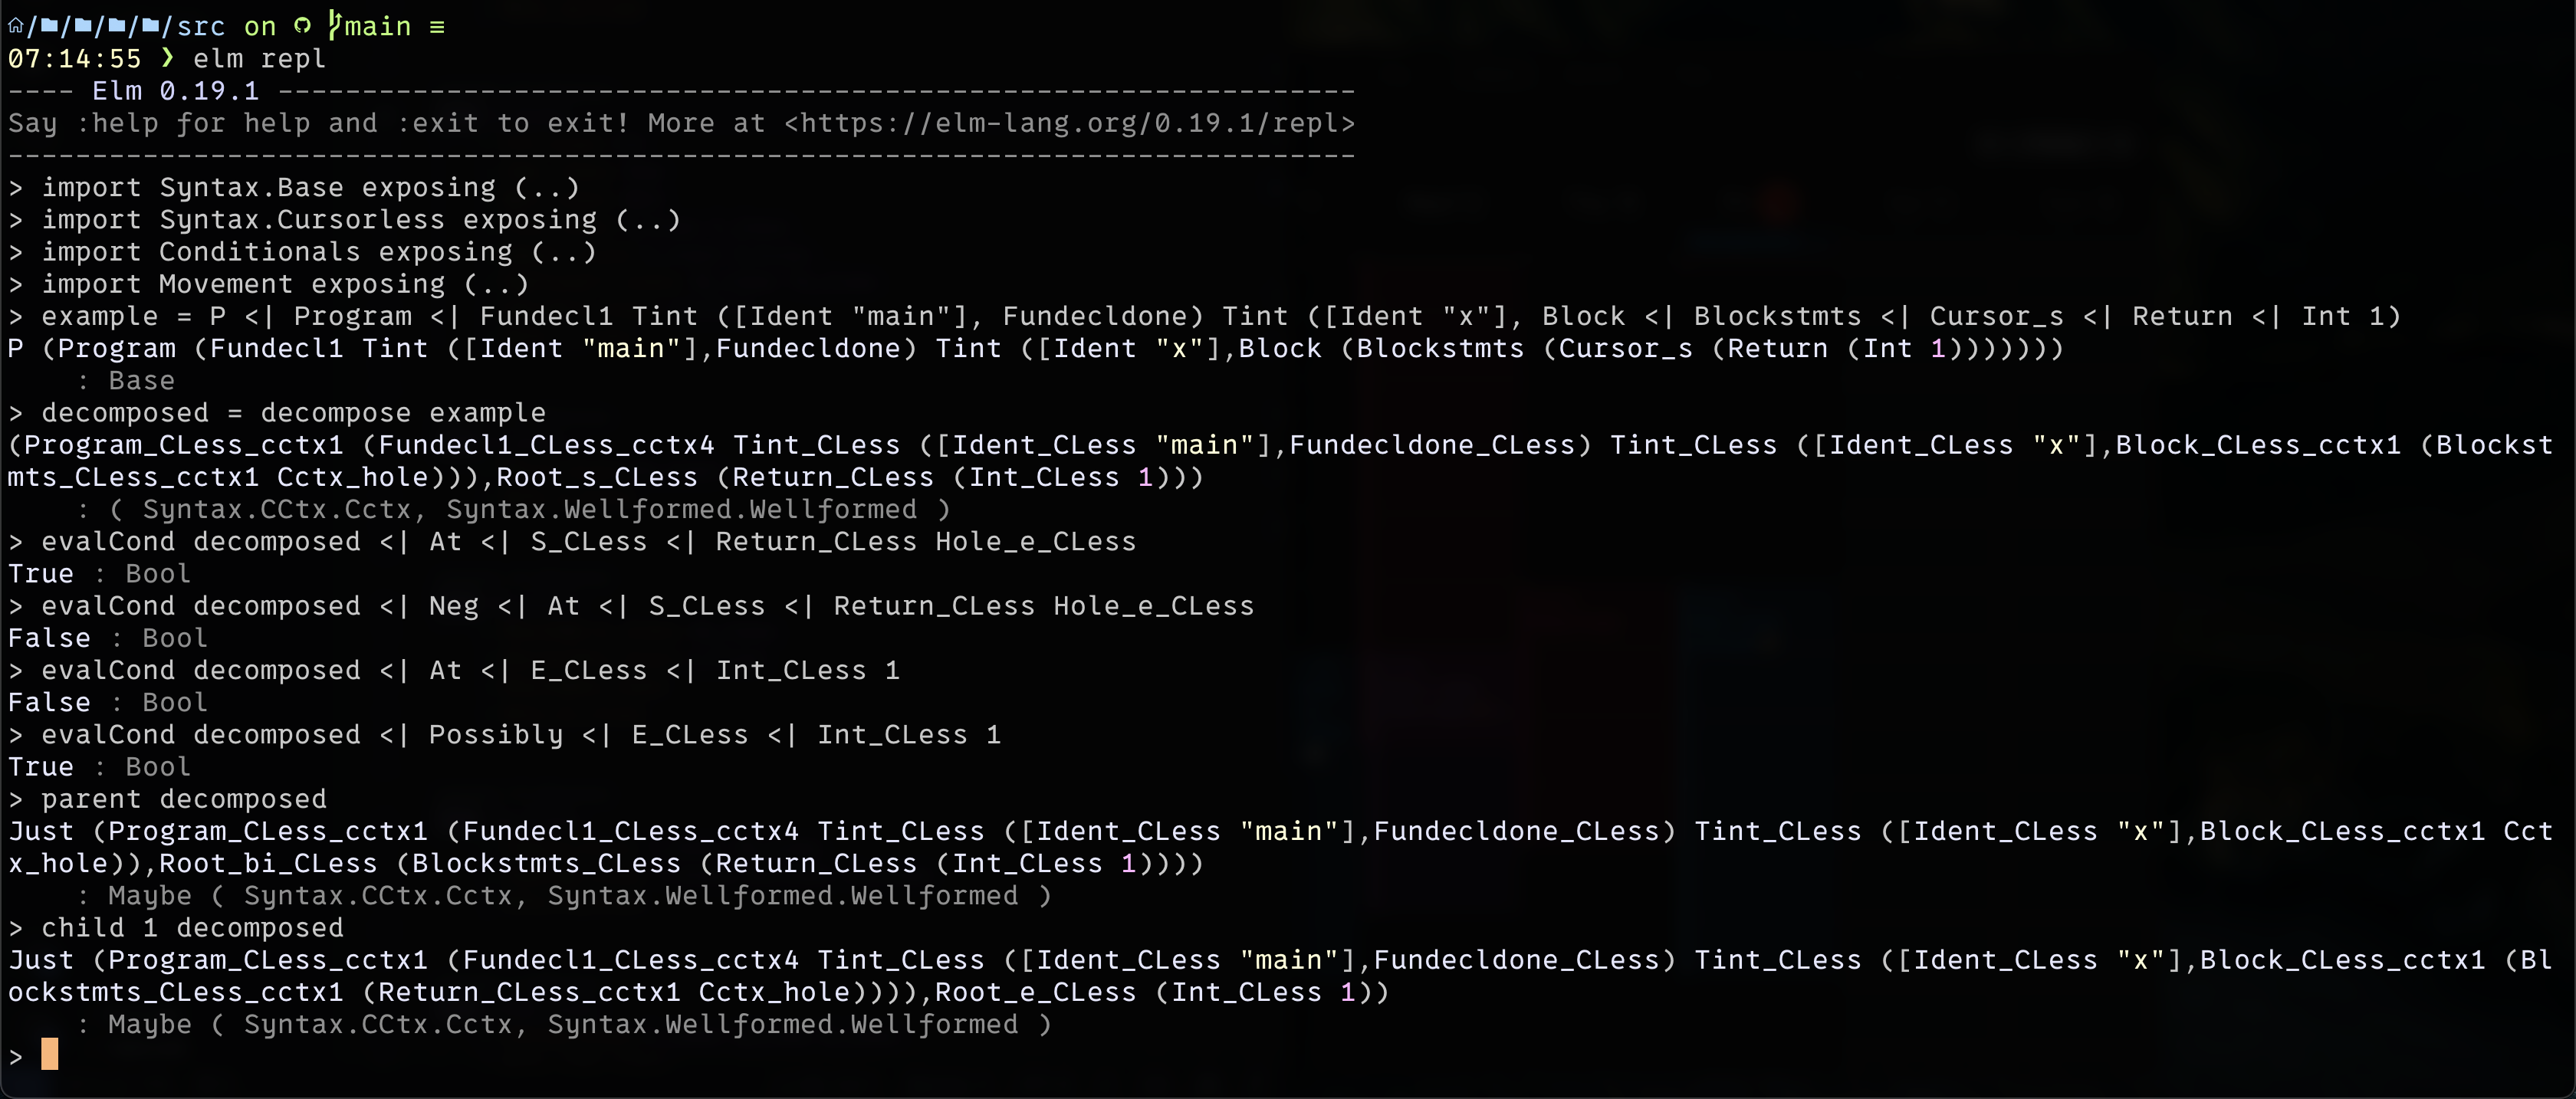
\includegraphics[width=\textwidth]{img/repl-editor.png}
\end{frame}


\begin{frame}[hvid]
    \frametitle{Implementation}
    \begin{itemize}
        \item Representing syntax
        \item Code generation vs. generic model
        \item Generating source code
        \item Editor expressions
    \end{itemize}
\end{frame}

\begin{frame}[hvid]
    \frametitle{Representing syntax}
    \begin{itemize}
        \item Abstract syntax per Robert Harper\footcite{harper}
              \begin{itemize}
                  \item Set of sorts $\mathcal{S}$
                  \item Arity-indexed family of operators $\mathcal{O}$
                  \item Sort-indexed family of variables $\mathcal{X}$
                  \item Binders: $(\vec{x_1}.x_1)s$
              \end{itemize}
              \pause
        \item How can a user provide this in a non-challenging way?
    \end{itemize}
\end{frame}

\begin{frame}
    \frametitle{Representing syntax (Continued)}
    \begin{itemize}
        \item Metal\footcite{metal}
        \pause
        \item Zephyr ASDL\footcite{zephyr}
        \pause
        \item ASN.1\footcite{asn1}
              \pause
        \item Common problem: no support for binders
    \end{itemize}
\end{frame}

\begin{frame}
    \frametitle{Representing syntax (Continued)}
    \begin{multicols}{2}
        \begin{itemize}
            \item Let's make our own specification language
                  \vspace{1cm}

                  \includegraphics<2->[width=0.45\textwidth]{img/spec-lang-parseable-ex.png}
        \end{itemize}

        \columnbreak
        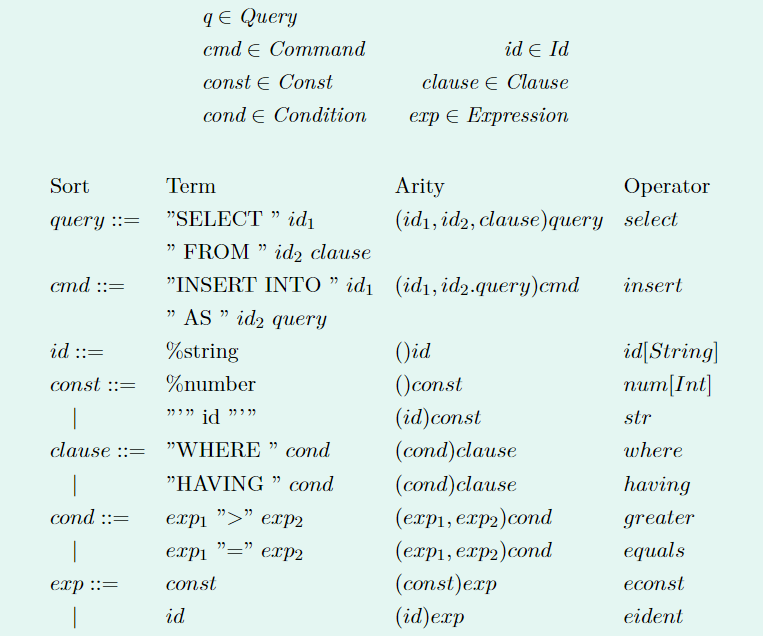
\includegraphics[width=0.5\textwidth]{img/spec-lang-ex.png}
    \end{multicols}

\end{frame}

\begin{frame}[hvid]
    \frametitle{Code generation or generic model?}
\end{frame}

\begin{frame}[hvid]
    \frametitle{Generating source code}
    \begin{itemize}
        \item Elm CodeGen package\footcite{elm-codegen-package}
    \end{itemize}
\end{frame}

\begin{frame}[hvid]
    \frametitle{Editor examples}
    \begin{itemize}
        \item C
        \item SQL
        \item \LaTeX
    \end{itemize}
\end{frame}


\begin{frame}[hvid]
    \frametitle{C}
\end{frame}

\begin{frame}[hvid]
    \frametitle{SQL}
\end{frame}

\begin{frame}[hvid]
    \frametitle{\LaTeX}
\end{frame}

\begin{frame}[hvid]
    \frametitle{Future work}

    \begin{itemize}
        \item
    \end{itemize}
\end{frame}



\begin{frame}[hvid]
    \frametitle{}
    \centering
    \large{Thank you for your attention!}
\end{frame}

\end{document}